\section{Key new insight}
\label{sec_key_new_insight}

1) In Fig.~\ref{fig_alphaVSber}, error propagation in existing 
NOMA PHY techniques (SIC) due to successive decoding of multiplexed 
signals needs to be taken into consideration in the simulation model.
As In the theoretical model, the data of previous stages can be 
fully decoded regarless of the power allocation.
2) The impact of modulation/coding scheme (MCS) selection as
well as the power allocation factor (PAF) among NOMA users
(users that share the same resource block) also needs to be taken
into consideration in the simulation model.
3) For a two-user NOMA system, pairing of users for sharing each
resource block should ensure that the bit error rates (BERs)
achieved at each user are within the tolerable range when the sum
rate is being maximized.

\begin{figure}[t]
\begin{center}
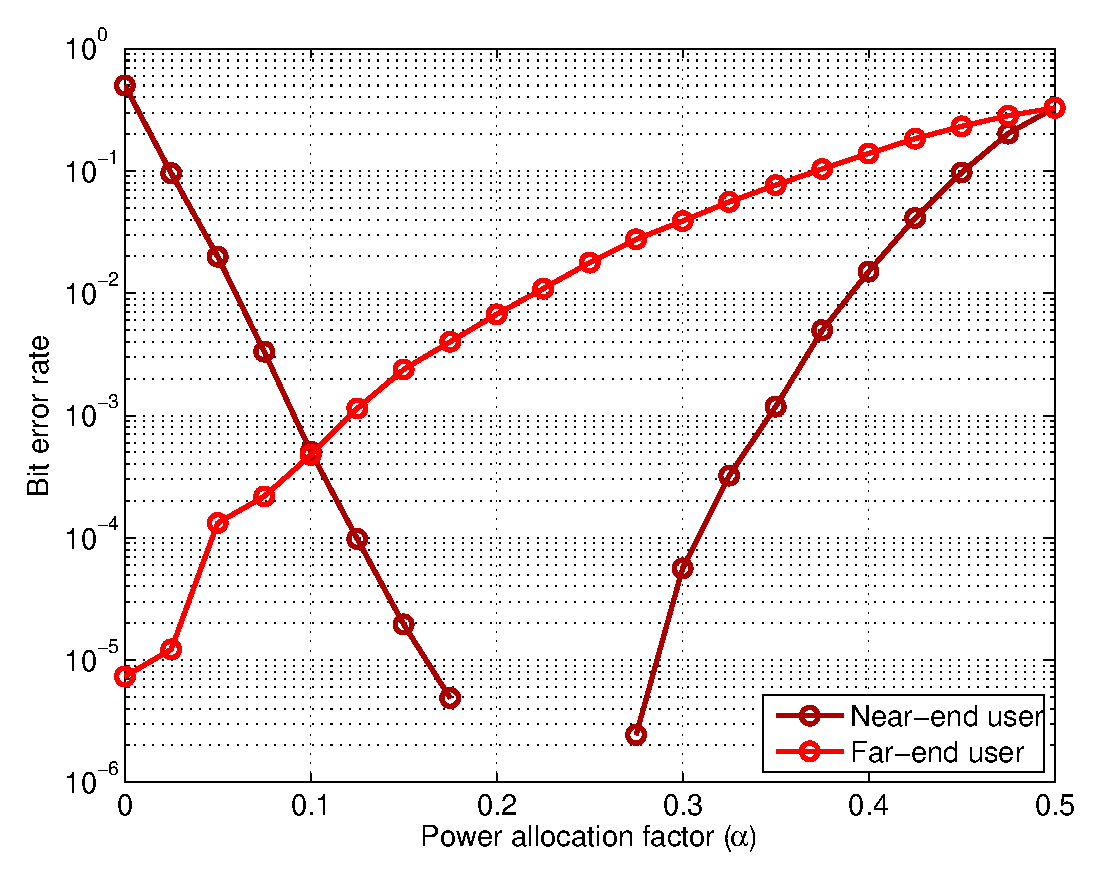
\includegraphics[width=0.9\columnwidth ,angle=0]{figure/alphaVSber.eps}
\caption{BER for different power allocation factor}
\label{fig_alphaVSber}
\end{center}
\end{figure}

